% Slides for 2025-07-22
% To create a slide, use the following:
% \begin{frame}{TITLE}
%     BODY
% \end{frame}

% To create a slide with a bullet list, use the following:
% \begin{frame}{TITLE}
%     \begin{itemize}
%         \item ITEM 1
%         \item ITEM 2
%     \end{itemize}    
% \end{frame}

% To create a slide with numbered list, use the following:
% \begin{frame}{TITLE}
%     \begin{enumerate}
%         \item ITEM 1
%         \item ITEM 2
%     \end{enumerate}
% \end{frame}

% To create a slide with a graphic:
% 1. Add the graphic to this folder (named picture.png)
% 2. Use the following:
% \begin{frame}{TITLE}
%     \centering
%     \includegraphics[height=0.7\textheight,width=0.7\textwidth,keepaspectratio]{picture.png}
% \end{frame}

% To create a slide with two columns, use the following:
% \begin{frame}{TITLE}
%     \begin{columns}
%         \begin{column}{0.5\textwidth}
%             COLUMN 1 BODY
%         \end{column}
%         \begin{column}{0.5\textwidth}
%             COLUMN 2 BODY
%         \end{column}
%     \end{columns}
% \end{frame}

\begin{frame}{ML Team Agenda}
    \begin{itemize}
        \item EGCI work
        \item Spectrogram visualization
        \item Grad-CAM
        \item Williams et al., 2025
        \item Whale detection
        \item Template matching
        \item Next steps
    \end{itemize}
\end{frame}

\begin{frame}{EGCI Work}
    \begin{figure}
        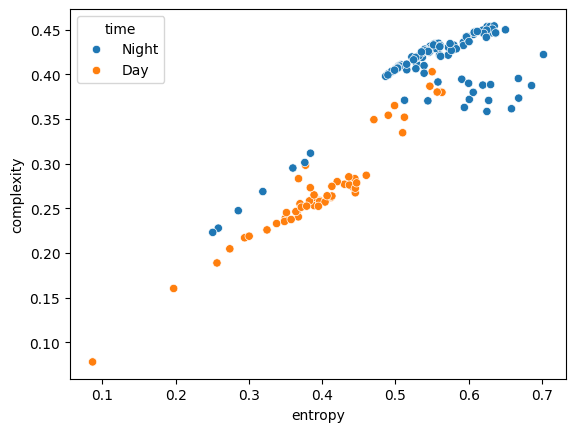
\includegraphics[height=0.7\textheight,width=0.7\textwidth,keepaspectratio]{images/muha_egci.png}
        \caption{Plot of EGCI against entropy for Muha's data, labeled with time of day}
    \end{figure}
\end{frame}

\begin{frame}{Spectrogram Visualization}
    High-dimensional spatial representation of audio clips
    \begin{figure}
        \centering
        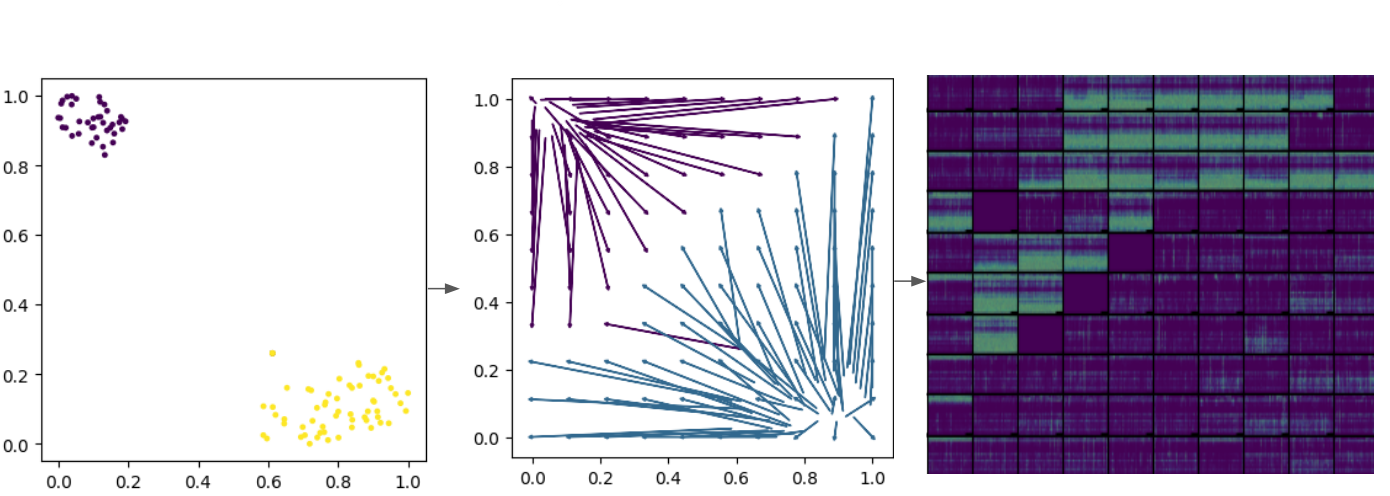
\includegraphics[height=0.85\textheight,width=0.85\textwidth,keepaspectratio]{images/spectrogram_visualization.png}
        \caption{Spectrogram visualization process of audio clips}
    \end{figure}
\end{frame}

\begin{frame}{Grad-CAM}
    \begin{columns}
        \begin{column}{0.5\textwidth}
            Degraded Grad-CAM:
            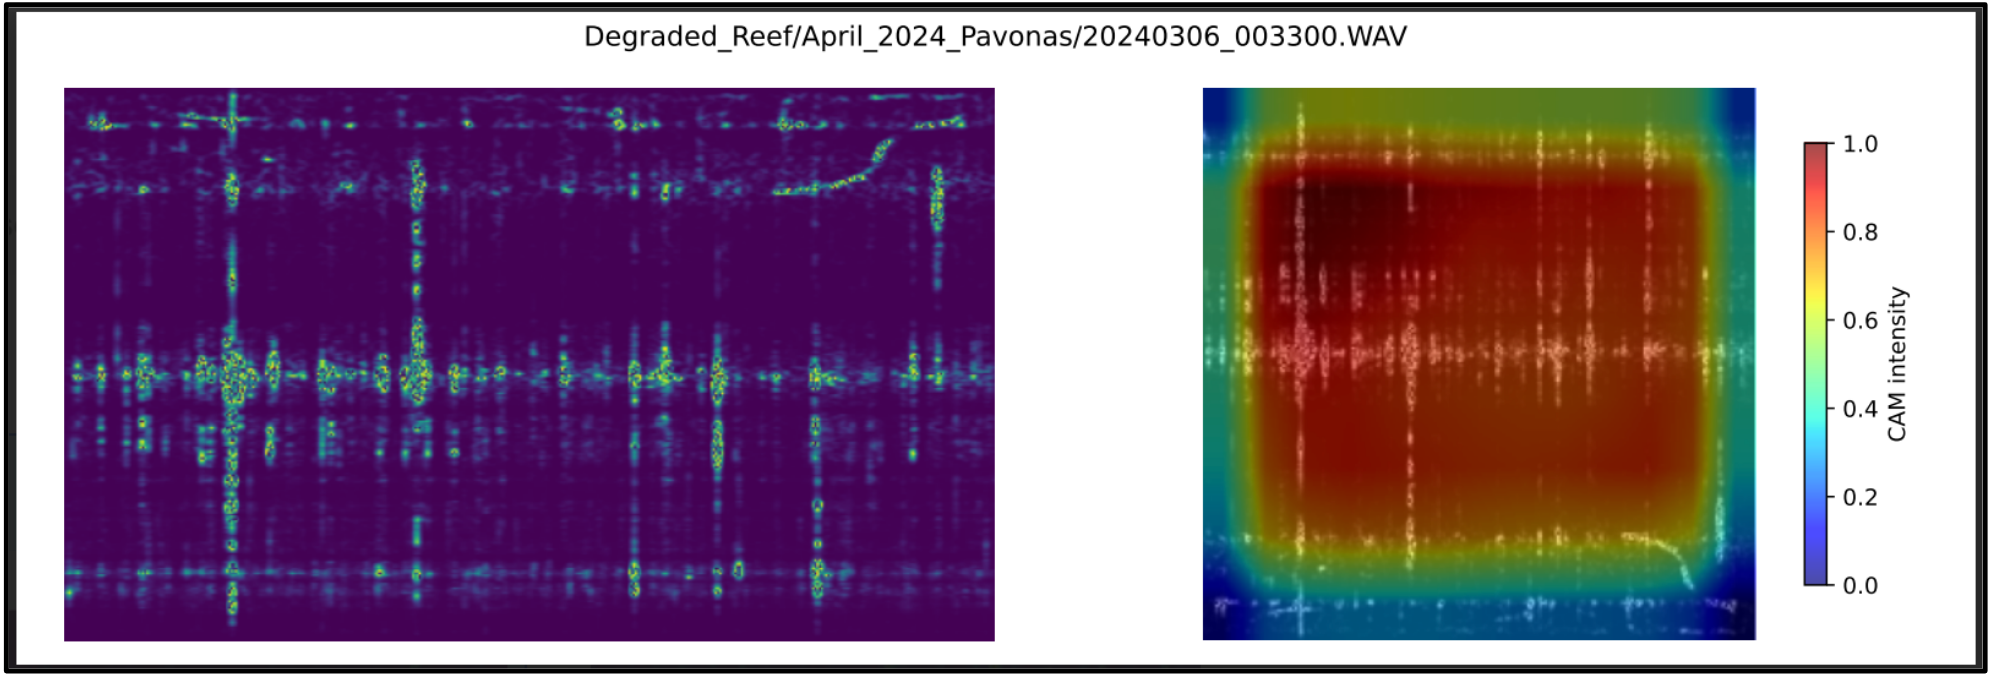
\includegraphics[height=1.0\textheight,width=1.0\textwidth,keepaspectratio]{images/degraded_grad_cam.png}
        \end{column}
        \begin{column}{0.5\textwidth}
            Non-degraded Grad-CAM:
            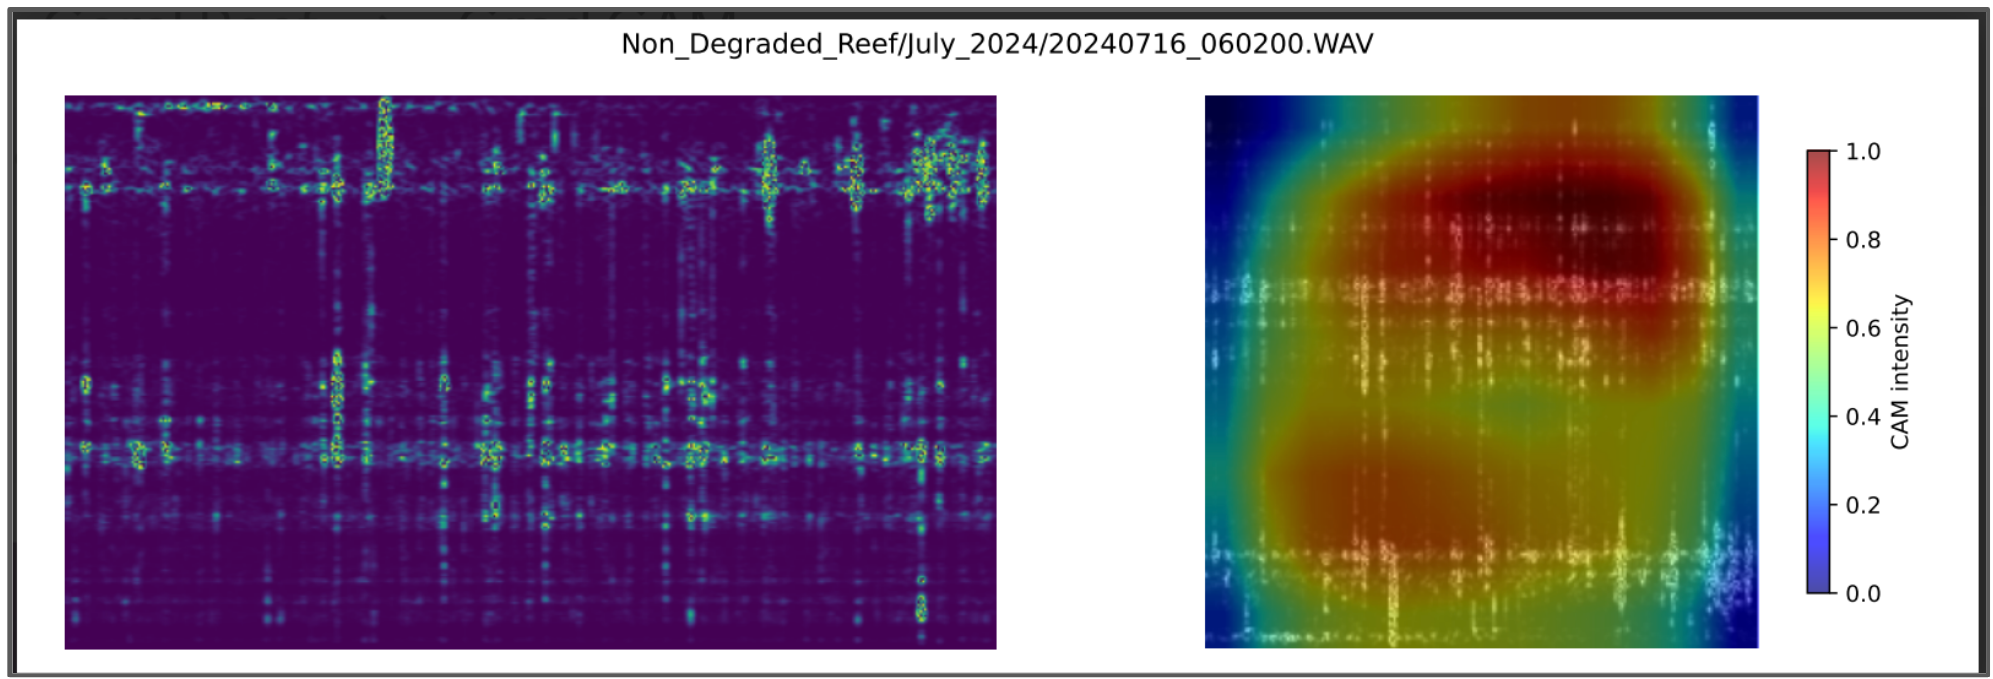
\includegraphics[height=1.0\textheight,width=1.0\textwidth,keepaspectratio]{images/non_degraded_grad_cam.png}
        \end{column}
    \end{columns}
\end{frame}

\begin{frame}{Grad-CAM Results}
    Sample of 200 degraded and non-degraded audio clips
    \begin{figure}
        \centering
        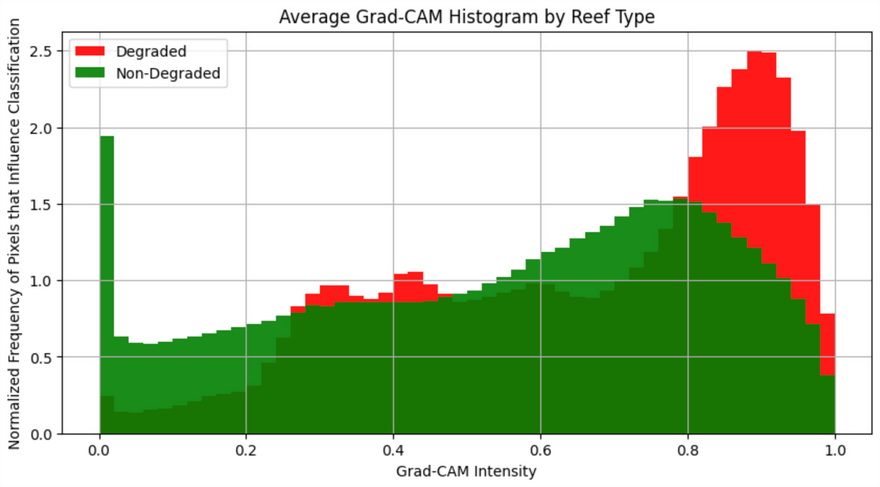
\includegraphics[height=0.6\textheight,width=0.6\textwidth,keepaspectratio]{images/grad_cam_histogram.png}
        \caption{Grad-CAM histogram}
    \end{figure}
\end{frame}

\begin{frame}{Williams et al., 2025}
    \begin{itemize}
        \item SurfPerch trained on worldwide reef sounds, tackles domain shift
        \item Using SurfPerch on Paola's data for knowledge discovery
    \end{itemize}
    \begin{columns}
        \begin{column}{0.5\textwidth}
            \begin{figure}
                \centering
                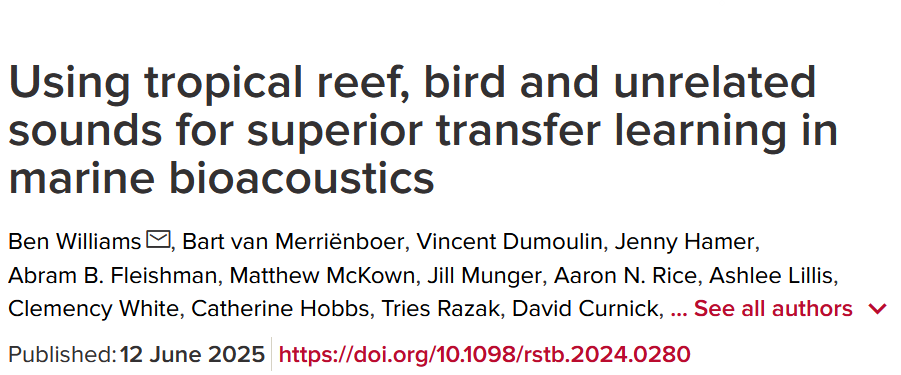
\includegraphics[height=0.8\textheight,width=0.8\textwidth,keepaspectratio]{images/Williams_et_al_2025.png}
            \end{figure}
        \end{column}
        \begin{column}{0.5\textwidth}
            \begin{figure}
                \centering
                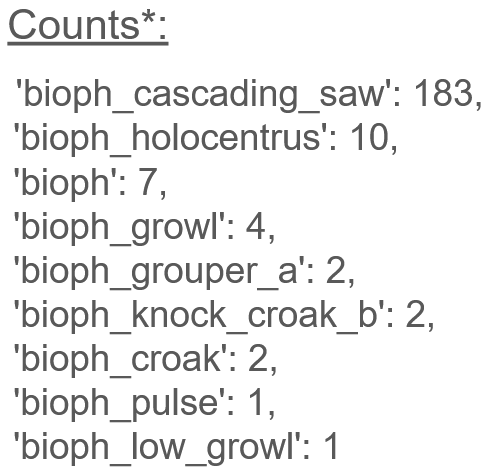
\includegraphics[height=0.5\textheight,width=0.5\textwidth,keepaspectratio]{images/surf_perch_results.png}
            \end{figure}
        \end{column}
    \end{columns}
    % Williams et al. 2025: https://royalsocietypublishing.org/doi/10.1098/rstb.2024.0280
    % SurfPerch: https://www.kaggle.com/models/google/surfperch
\end{frame}

\begin{frame}{Whale Detection}
    \begin{itemize}
        \item Can use multispecies-whale model to detect humpback whale vocalizations
        \item Issues quantifying accuracy, lack of ground truth
        \item 5\% of audio clips contain whale noises
    \end{itemize}
    \begin{figure}
        \centering
        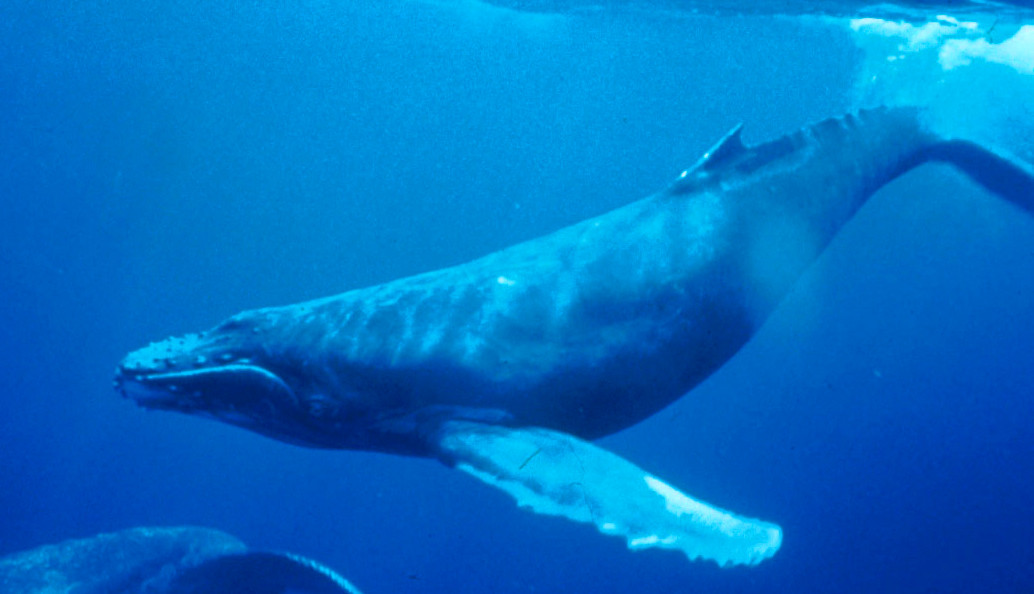
\includegraphics[height=0.4\textheight,width=0.4\textwidth,keepaspectratio]{images/humpback_whale.jpg}
        \caption{Humpback whale}
    \end{figure}
    % multispecies-whale model: https://www.kaggle.com/models/google/multispecies-whale
\end{frame}

\begin{frame}{Template Matching}
    \begin{itemize}
        \item Can take a template sound and find similar sounds in a dataset
        \item Works decently well, need to work on refinements
        \item Red-eyed dove example:
        \begin{columns}
            \begin{column}{0.5\textwidth}
                \begin{figure}
                    \centering
                    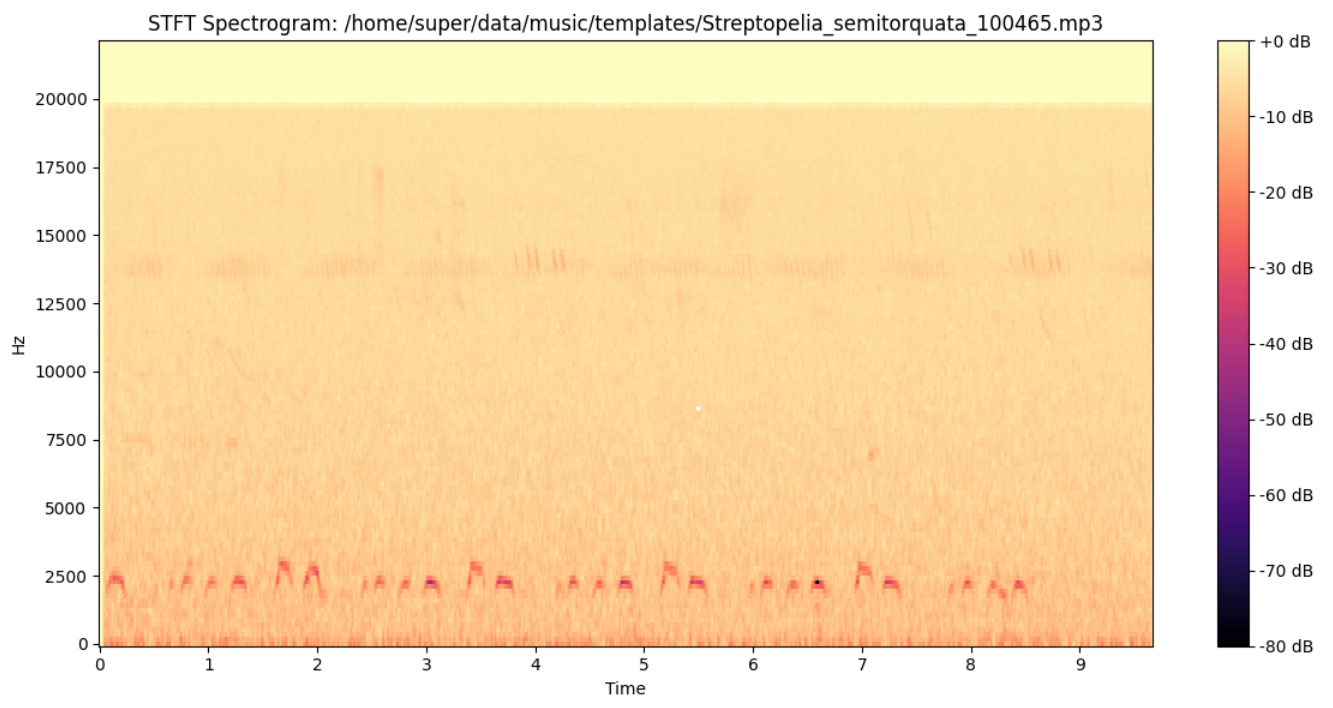
\includegraphics[height=1.0\textheight,width=1.0\textwidth,keepaspectratio]{images/dove_stft_spectrogram.png}
                \end{figure}
            \end{column}
            \begin{column}{0.5\textwidth}
                \begin{figure}
                    \centering
                    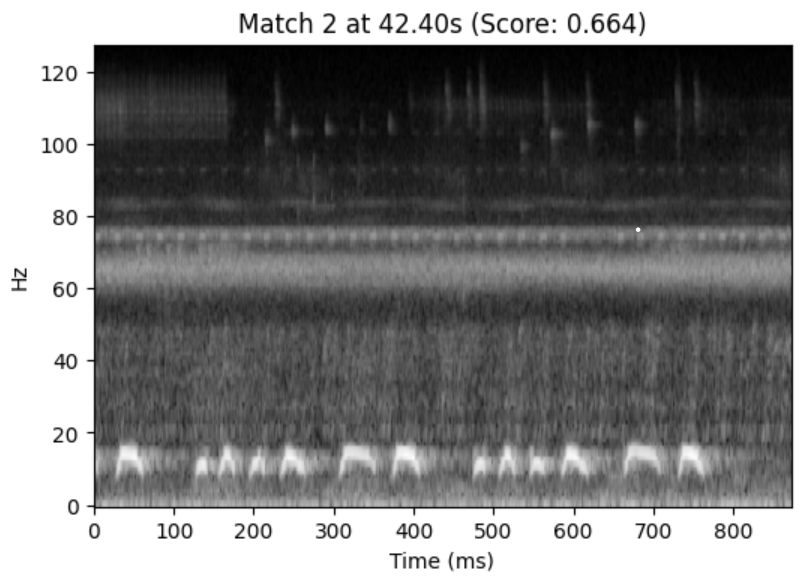
\includegraphics[height=0.8\textheight,width=0.8\textwidth,keepaspectratio]{images/template_matching_ex.png}
                \end{figure}
            \end{column}
        \end{columns}
    \end{itemize}
\end{frame}

\begin{frame}{Next Steps}
    \begin{itemize}
        \item Create interactive website for Muha with D3.js
        \item Further work on knowledge graphs (GNNs)
        \item Evaluate options for Paola
        \item Continue with template matching work
        \item Sound separation
    \end{itemize}
\end{frame}

\begin{frame}{Collar Team Agenda}
    \begin{itemize}
        \item Power Studies
        \begin{itemize}
            \item Power Study Overview
            \item Test Setup 
            \item In-rush Current Measurements
            \item Run Mode Configuration Measurements
        \end{itemize}
        \item Data Loss
        \begin{itemize}
            \item What is bit rot?
            \item Types of NAND flash
            \item Maintaining data integrity
            \item Fermi estimations
            \item Lit Review: Possible solutions
            \item What's next?
        \end{itemize}
        \item Future Plans
    \end{itemize}
\end{frame}

\begin{frame}{Power Study Overview}
    \begin{itemize}
        \item Understand power behaviour of STM32H747I-DISCO
        \item Measure various runtime domains for collar design metrics
    \end{itemize}
\end{frame}

\begin{frame}{Test Setup}
    \begin{itemize}
        \item Measurements taken using current clamp
        \item Drift issue → 10 Ohms shunt resistor
        \item Current calculated using V\_high - V\_low / 10 Ohms
    \end{itemize}  
    \includegraphics[height=0.35\textheight,width=0.7\textwidth,keepaspectratio]{images/clamp_setup.png}
    \includegraphics[height=0.35\textheight,width=0.7\textwidth,keepaspectratio]{images/shunt_setup.png}
    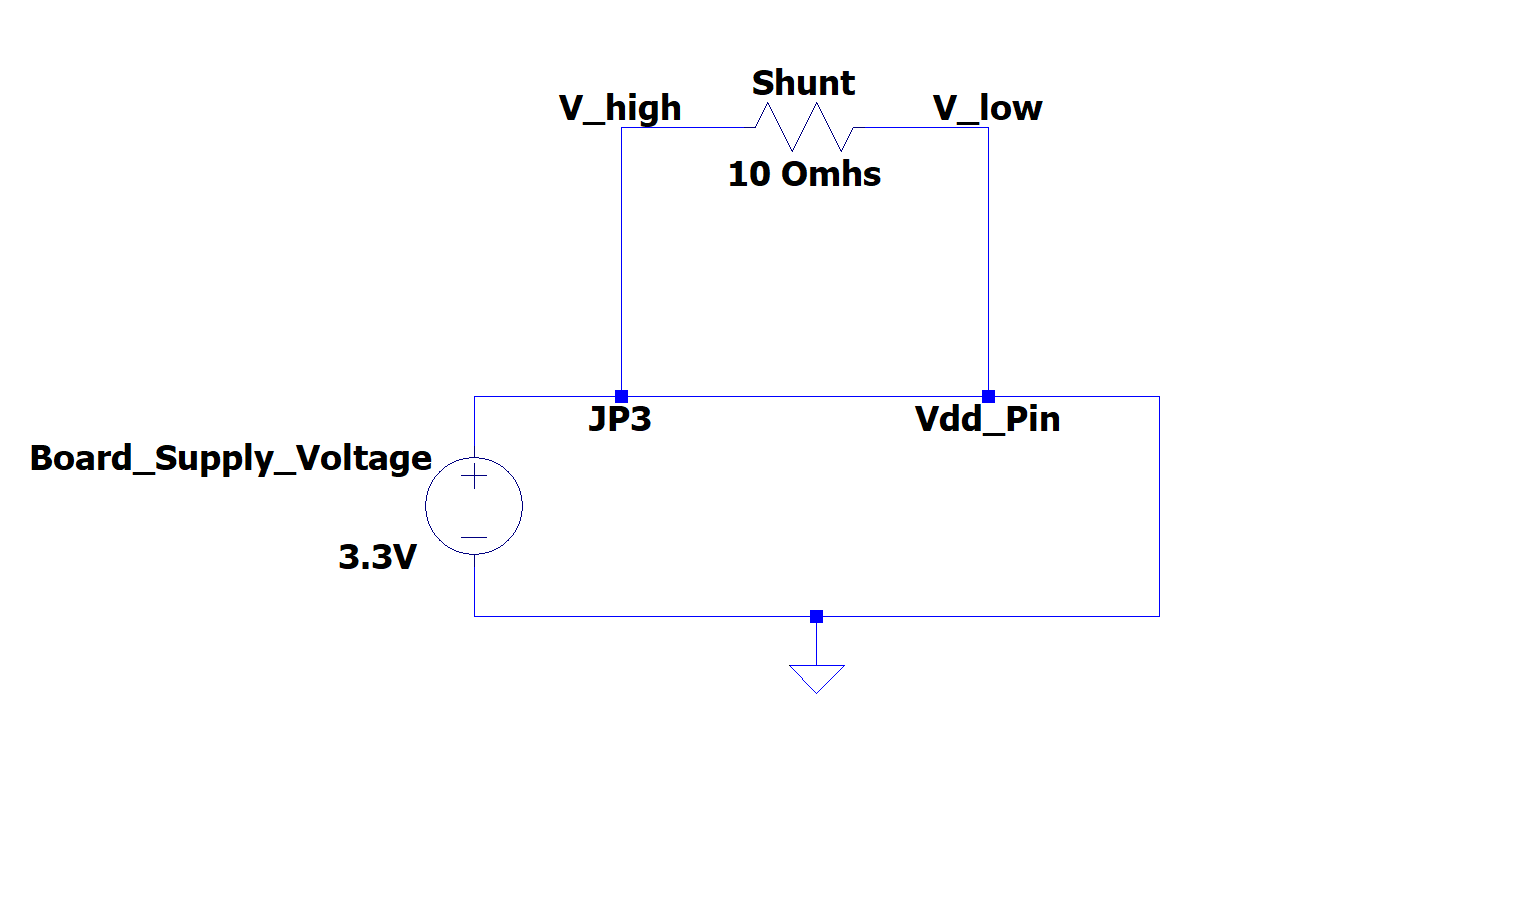
\includegraphics[height=0.35\textheight,width=0.7\textwidth,keepaspectratio]{images/shunt.png}
\end{frame}

\begin{frame}{In-Rush Current Measurements}
\begin{columns}

    % Left column: image
    \begin{column}{0.6\textwidth}
        \centering
        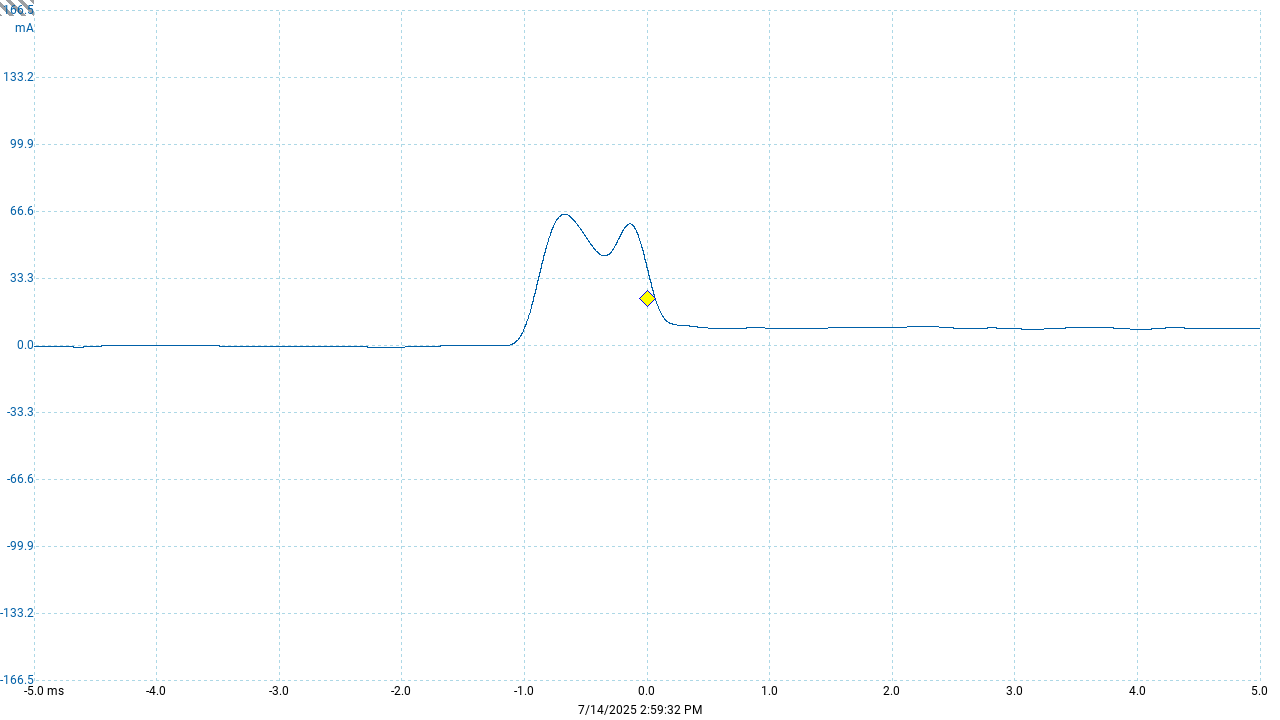
\includegraphics[width=\linewidth]{images/inrush_1core_baseline.png}
        \vspace{0.5em}
        {\small \textit{In-rush current spike at startup}}
    \end{column}

    % Right column: table
    \begin{column}{0.45\textwidth}
        \centering
        \begin{tabular}{|l|c|}
            \hline
            \textbf{Metric} & \textbf{Value} \\
            \hline
            Avg In-rush Peak 1 & 63.53 mA \\
            Avg In-rush Trough & 42.46 mA \\
            Avg In-rush Peak 2 & 58.27 mA \\
            Avg Duration     & 1.20 ms \\
            Method           & Current Clamp \\
            Trials           & 5 \\
            \hline
        \end{tabular}
        \vspace{0.5em}
        {\small \textit{In-rush Average Metrics}}
    \end{column}
\end{columns}
\end{frame}

\begin{frame}{Run Mode Configuration Measurements}
    \centering
    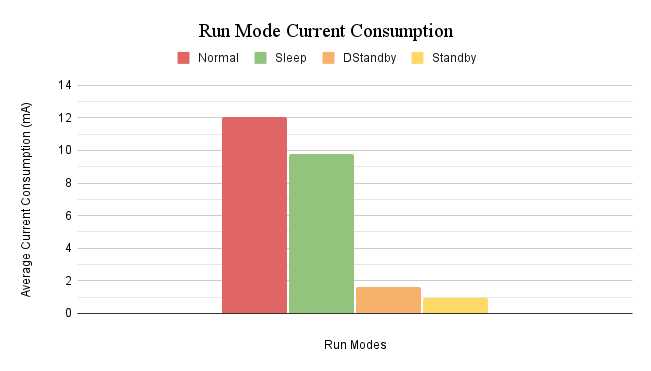
\includegraphics[height=0.8\textheight,width=1.0\textwidth,keepaspectratio]{images/run_modes.png}
\end{frame}

\begin{frame}{What is Bit Rot?}
    \begin{itemize}
        \item Digital data slowly corrupting overtime
        \item It occurs when: hold voltage fluctuates, reading/writing, storage wears out
    \end{itemize}
    \centering
    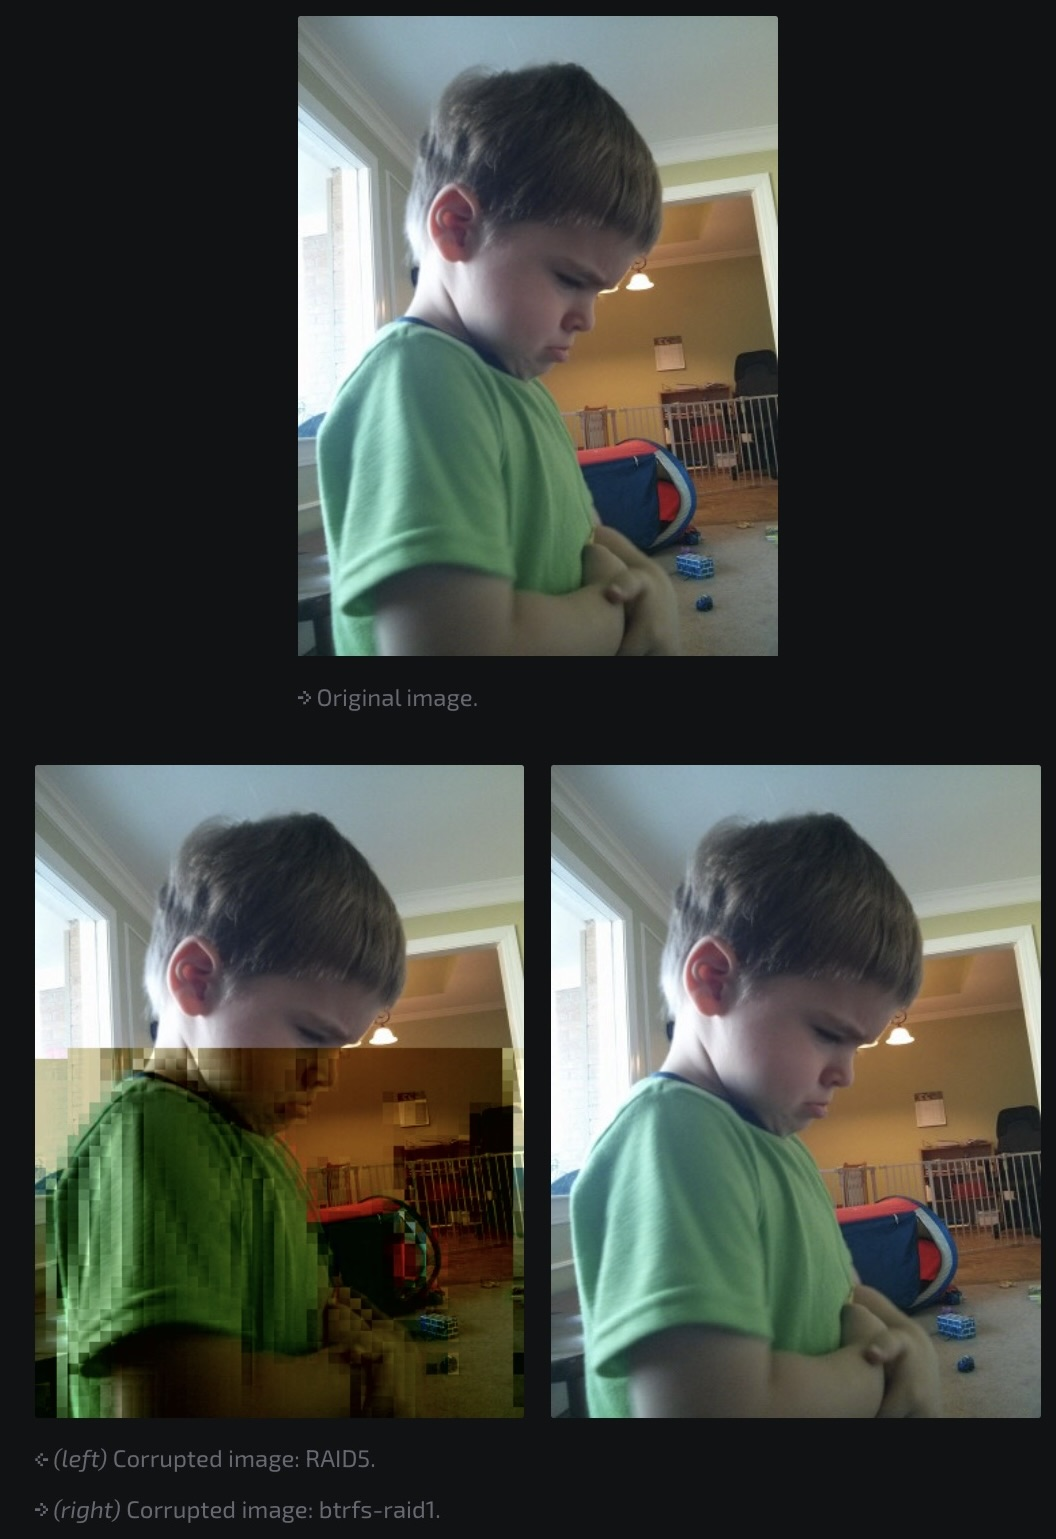
\includegraphics[height=0.7\textheight,width=0.7\textwidth,keepaspectratio]{images/bit_flip.png}
\end{frame}

\begin{frame}{Types of NAND Flash}
    \centering
    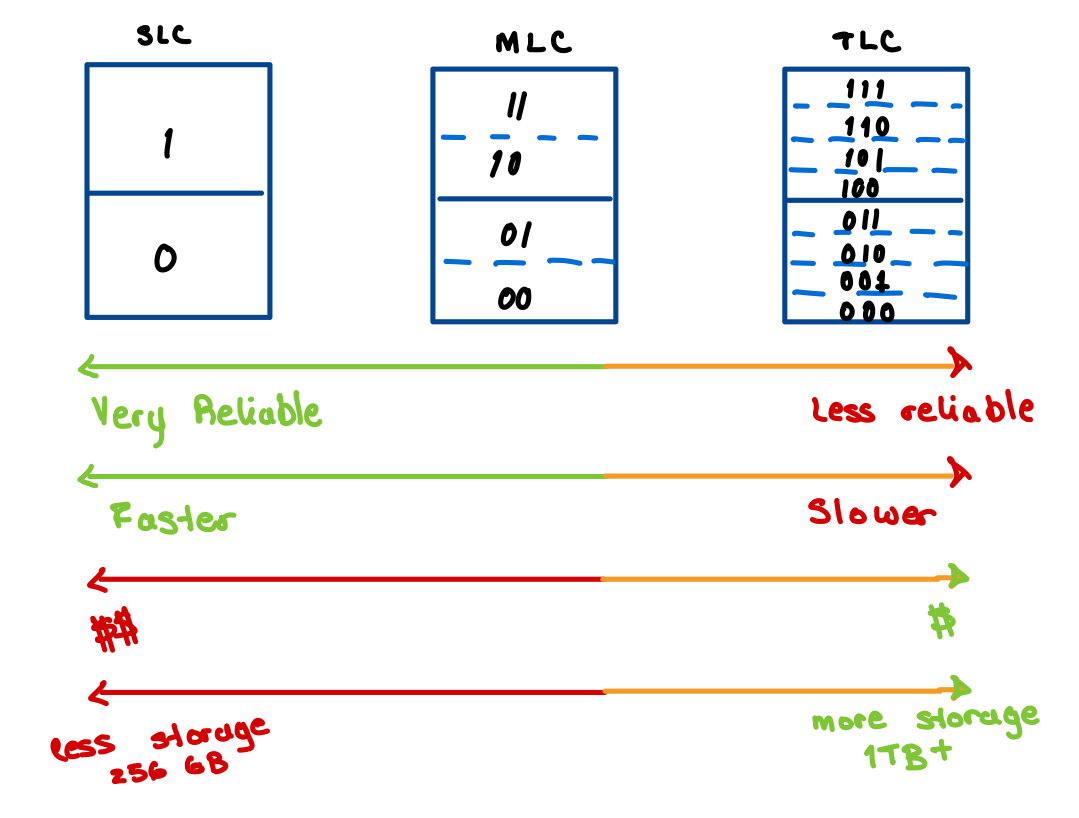
\includegraphics[height=0.9\textheight,width=0.9\textwidth,keepaspectratio]{images/flash_types.png}
\end{frame}

\begin{frame}{Maintaining Data Integrity}
    Managing data loss on three levels:
    \begin{itemize}
        \item \textbf{Hardware:} Use of ECC (Error-Correcting Code), choice of NAND flash type
        \item \textbf{File System:} Use of error checking file systems eg. ZFS, ext4
        \item \textbf{File/Page:} Use of checksums and hashes
    \end{itemize}
\end{frame}

\begin{frame}{Fermi Estimations}
    \begin{columns}
        \begin{column}{0.5\textwidth}
            \begin{figure}
                \centering
                \includegraphics[height=0.9\textheight,width=0.9\textwidth,keepaspectratio]{images/fermi_estimation.png}
                \caption{Fermi estimation of storage and power requirements}
            \end{figure}
       \end{column}
        \begin{column}{0.5\textwidth}
            \begin{itemize}
            \item \textbf{SD card size:} $\ge1*10^2$ GB
            \item \textbf{Battery:} 3-4 lbs
            \end{itemize}
            *Overhead to consider: compressing files to .flac, power fail safe
        \end{column}
    \end{columns}
\end{frame}

\begin{frame}{Lit Review: Possible Solutions}
    \begin{columns}
        \begin{column}{0.5\textwidth}
            \begin{itemize}
                \item \textbf{Error-Correcting Codes (ECC):} Detect and correct errors in data
            \end{itemize}
        \end{column}
        \begin{column}{0.5\textwidth}
            \begin{figure}
                \centering
                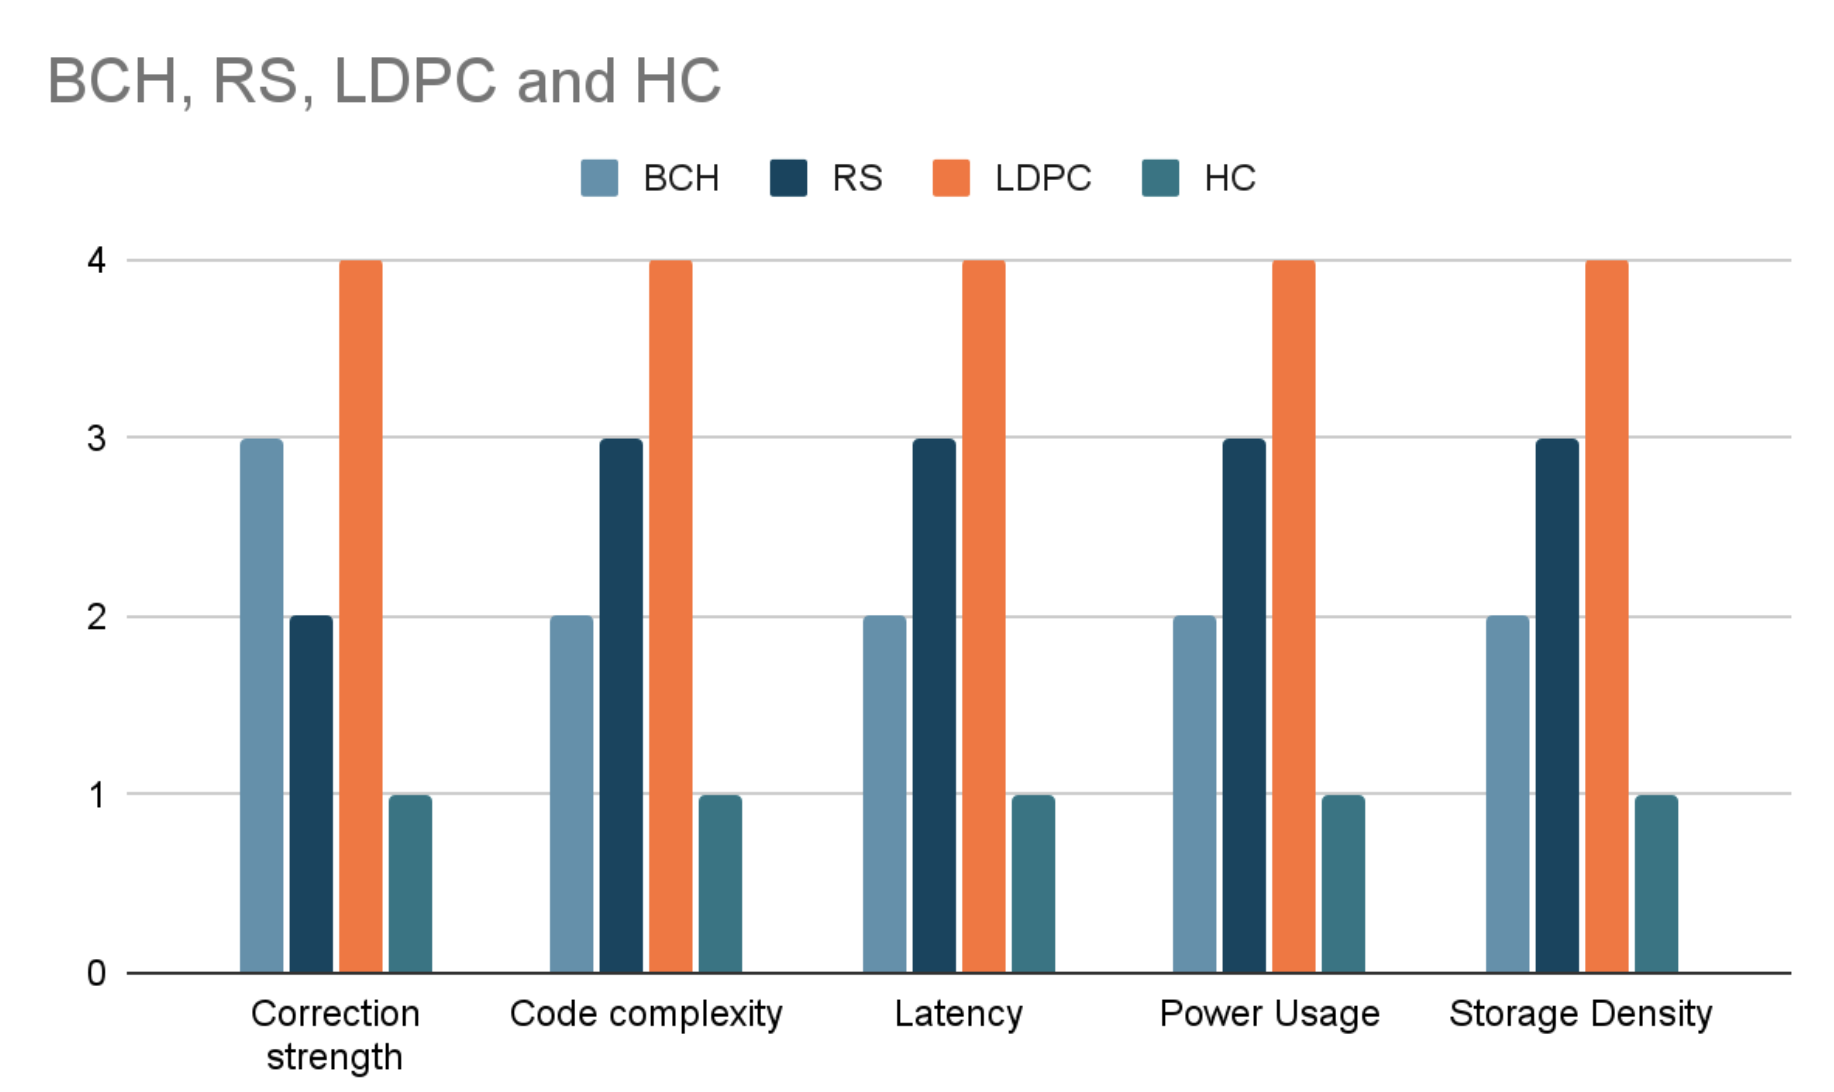
\includegraphics[height=0.5\textheight,width=0.6\textwidth,keepaspectratio]{images/ecc.png}
                \caption{Ranking of ECC (based on lit review)}
            \end{figure}
        \end{column}
    \end{columns}  
\end{frame}

\begin{frame}{Lit Review: Possible Solutions}
    \begin{columns}
        \begin{column}{0.5\textwidth}
            \begin{itemize}
                \item \textbf{Error-Correcting Codes (ECC):} Detect and correct errors in data
            \end{itemize}
        \end{column}
        \begin{column}{0.5\textwidth}
            \begin{figure}
                \centering
                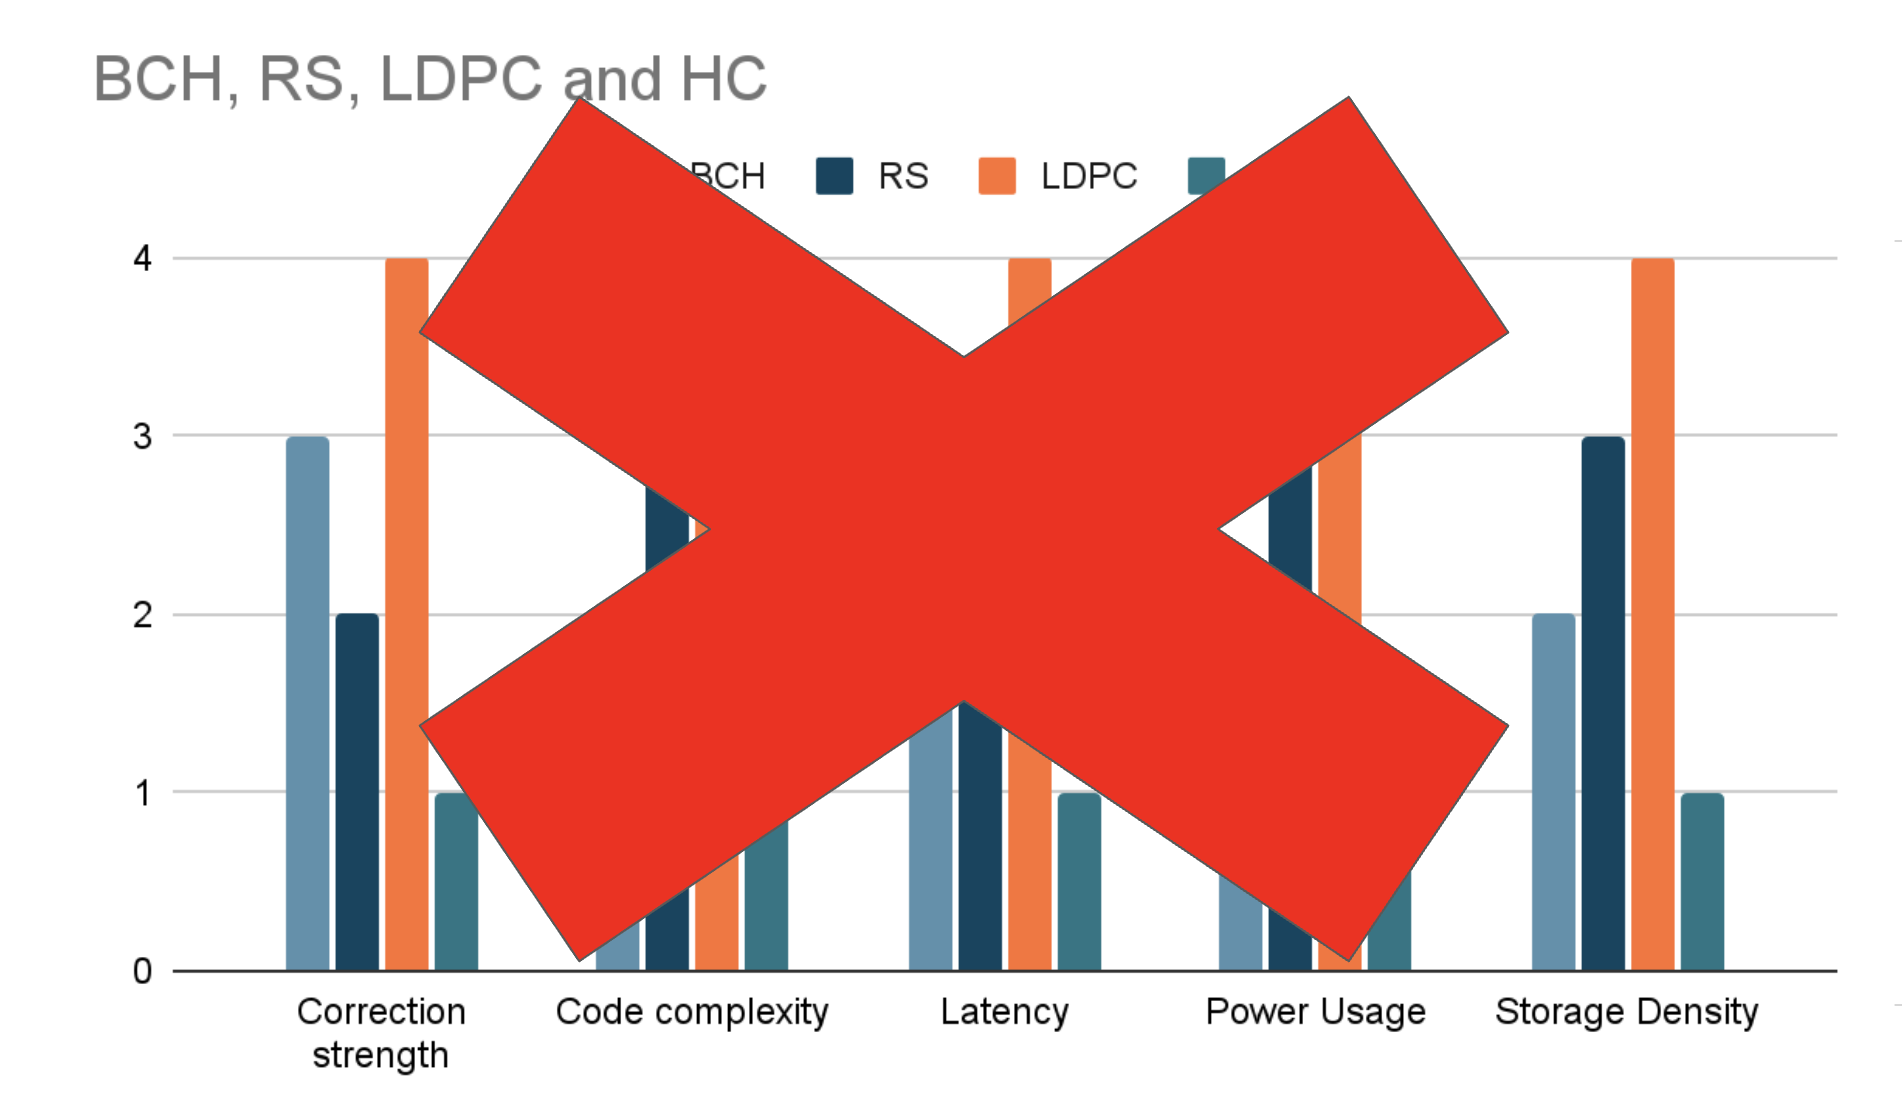
\includegraphics[height=0.5\textheight,width=0.6\textwidth,keepaspectratio]{images/ecc_x.png}
                \caption{Ranking of ECC (based on lit review)}
            \end{figure}
        \end{column}
    \end{columns}  
\end{frame}

\begin{frame}{Lit Review: Possible Solutions}
    \begin{columns}
        \begin{column}{0.5\textwidth}
            \begin{itemize}
                \item \textbf{Error-Correcting Codes (ECC):} Detect and correct errors in data
                \item \textbf{File System Integration:} Integrating SafeFAT or ZFS to manage data integrity
           \end{itemize}
        \end{column}
        \begin{column}{0.5\textwidth}
            \begin{figure}
                \centering
                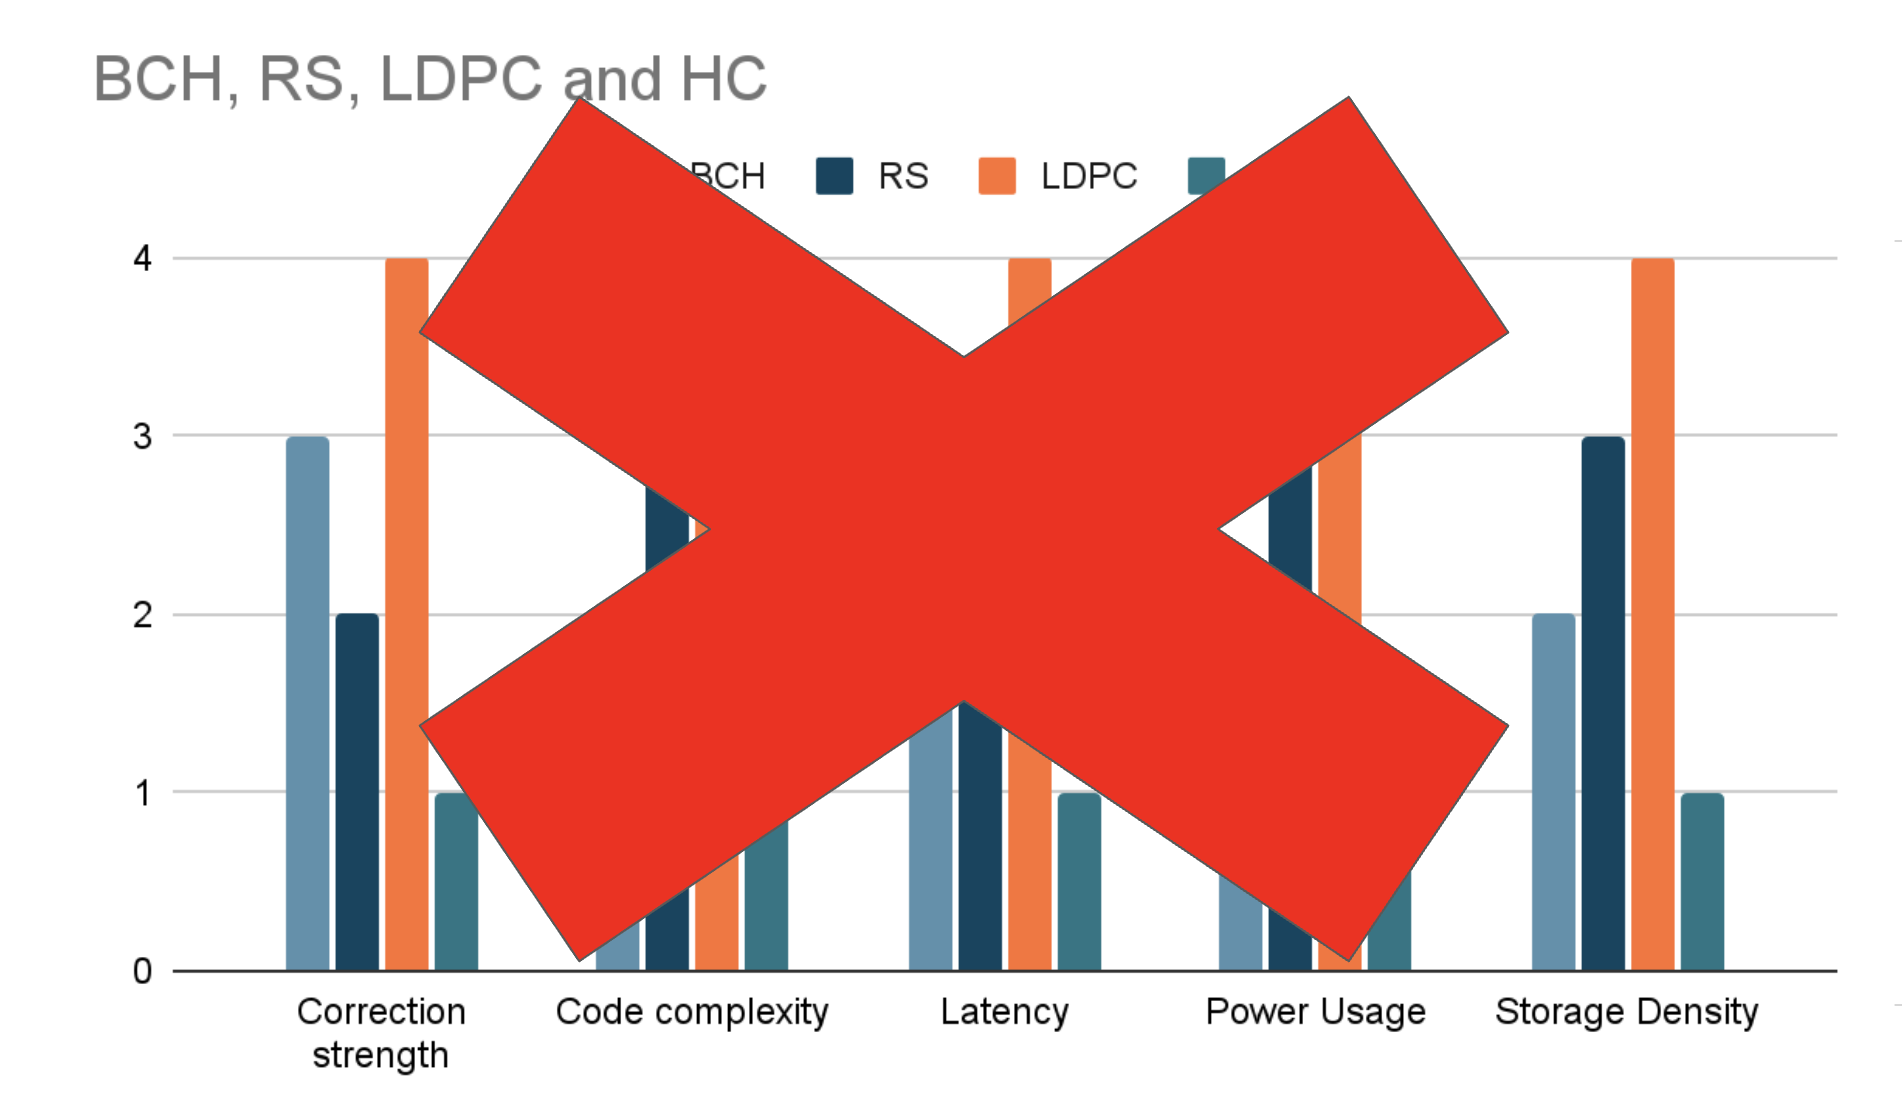
\includegraphics[height=0.4\textheight,width=0.5\textwidth,keepaspectratio]{images/ecc_x.png}
                \caption{Ranking of ECC (based on lit review)}
            \end{figure}
            \begin{figure}
                \centering
                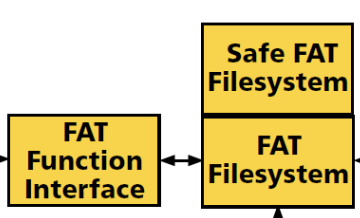
\includegraphics[height=0.5\textheight,width=0.6\textwidth,keepaspectratio]{images/safefat.png}
                \caption{SafeFAT integration}
            \end{figure}
        \end{column}
    \end{columns}  
\end{frame}

\begin{frame}{Lit Review: Possible Solutions}
    \begin{columns}
        \begin{column}{0.5\textwidth}
            \begin{itemize}
                \item \textbf{Error-Correcting Codes (ECC):} Detect and correct errors in data
                \item \textbf{File System Integration:} Integrating SafeFAT or ZFS to manage data integrity
           \end{itemize}
        \end{column}
        \begin{column}{0.5\textwidth}
            \begin{figure}
                \centering
                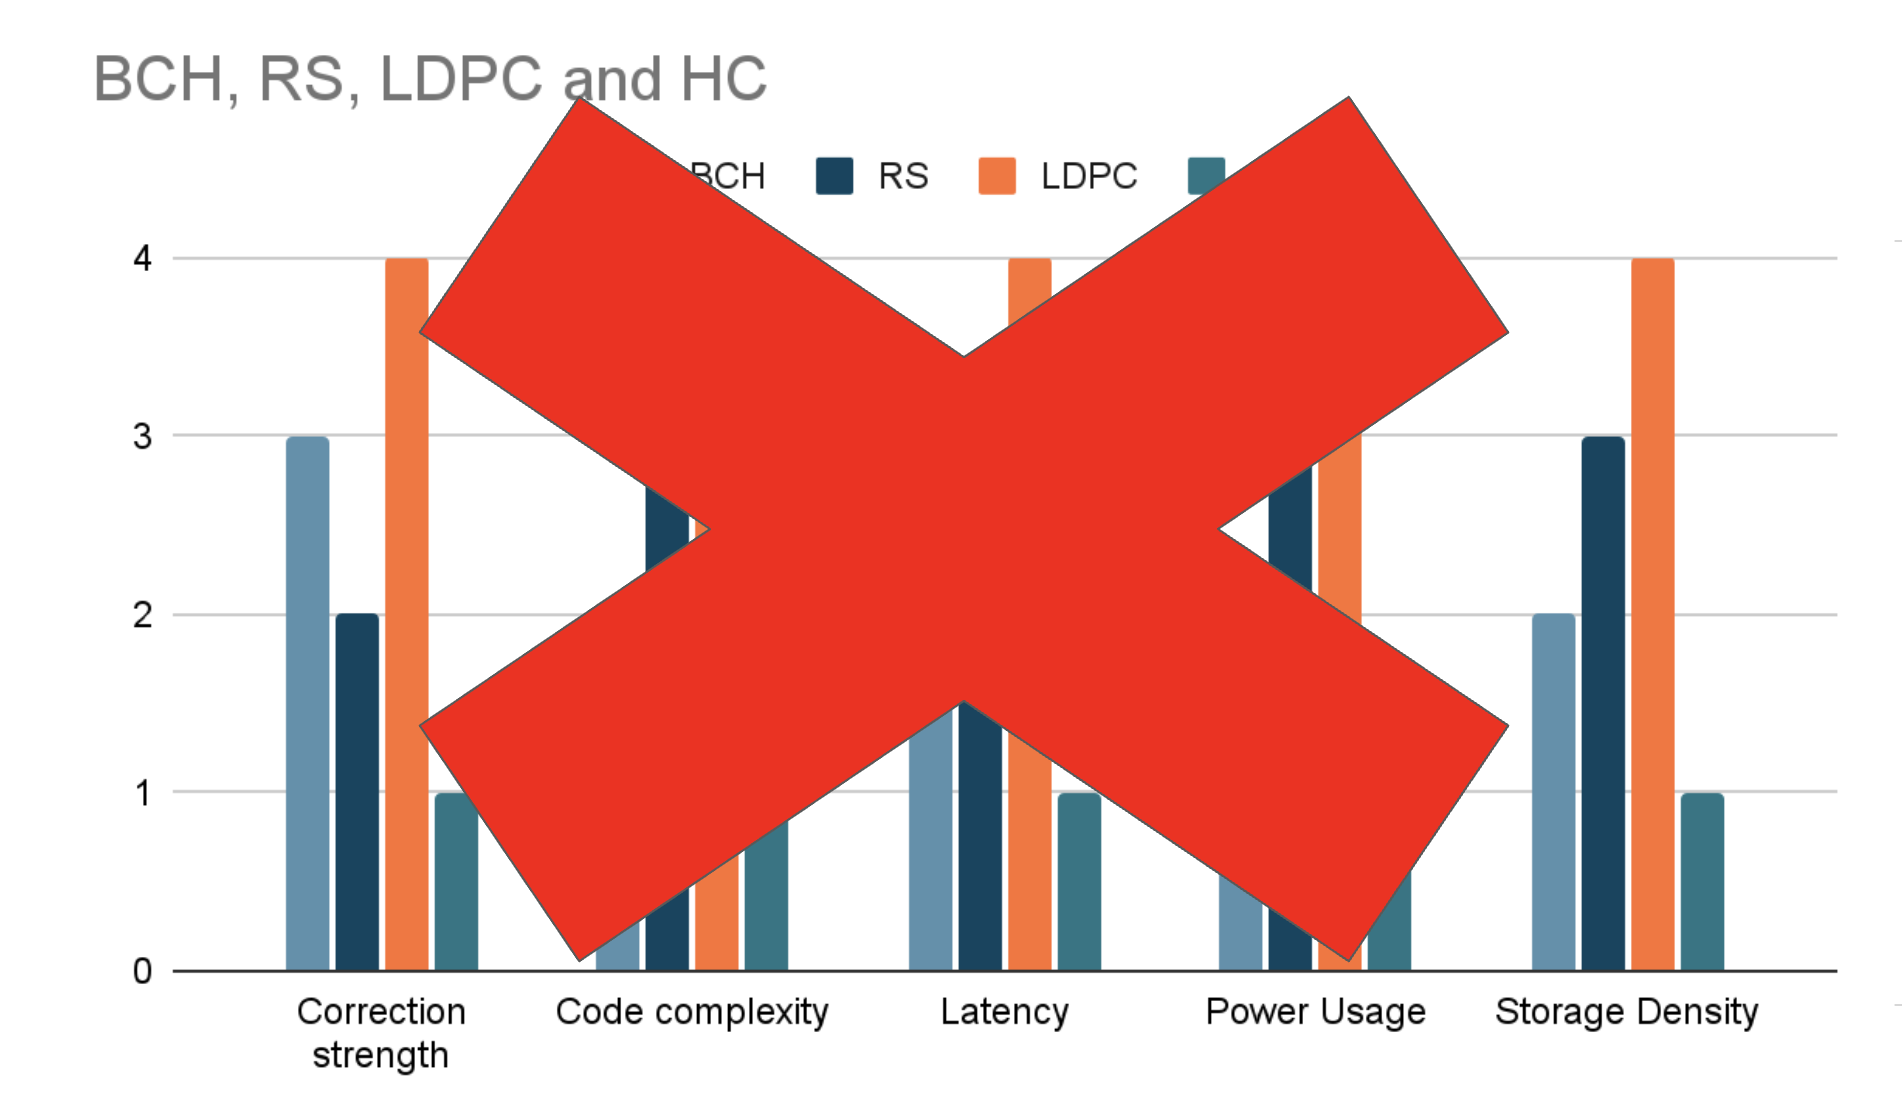
\includegraphics[height=0.4\textheight,width=0.5\textwidth,keepaspectratio]{images/ecc_x.png}
                \caption{Ranking of ECC (based on lit review)}
            \end{figure}
            \begin{figure}
                \centering
                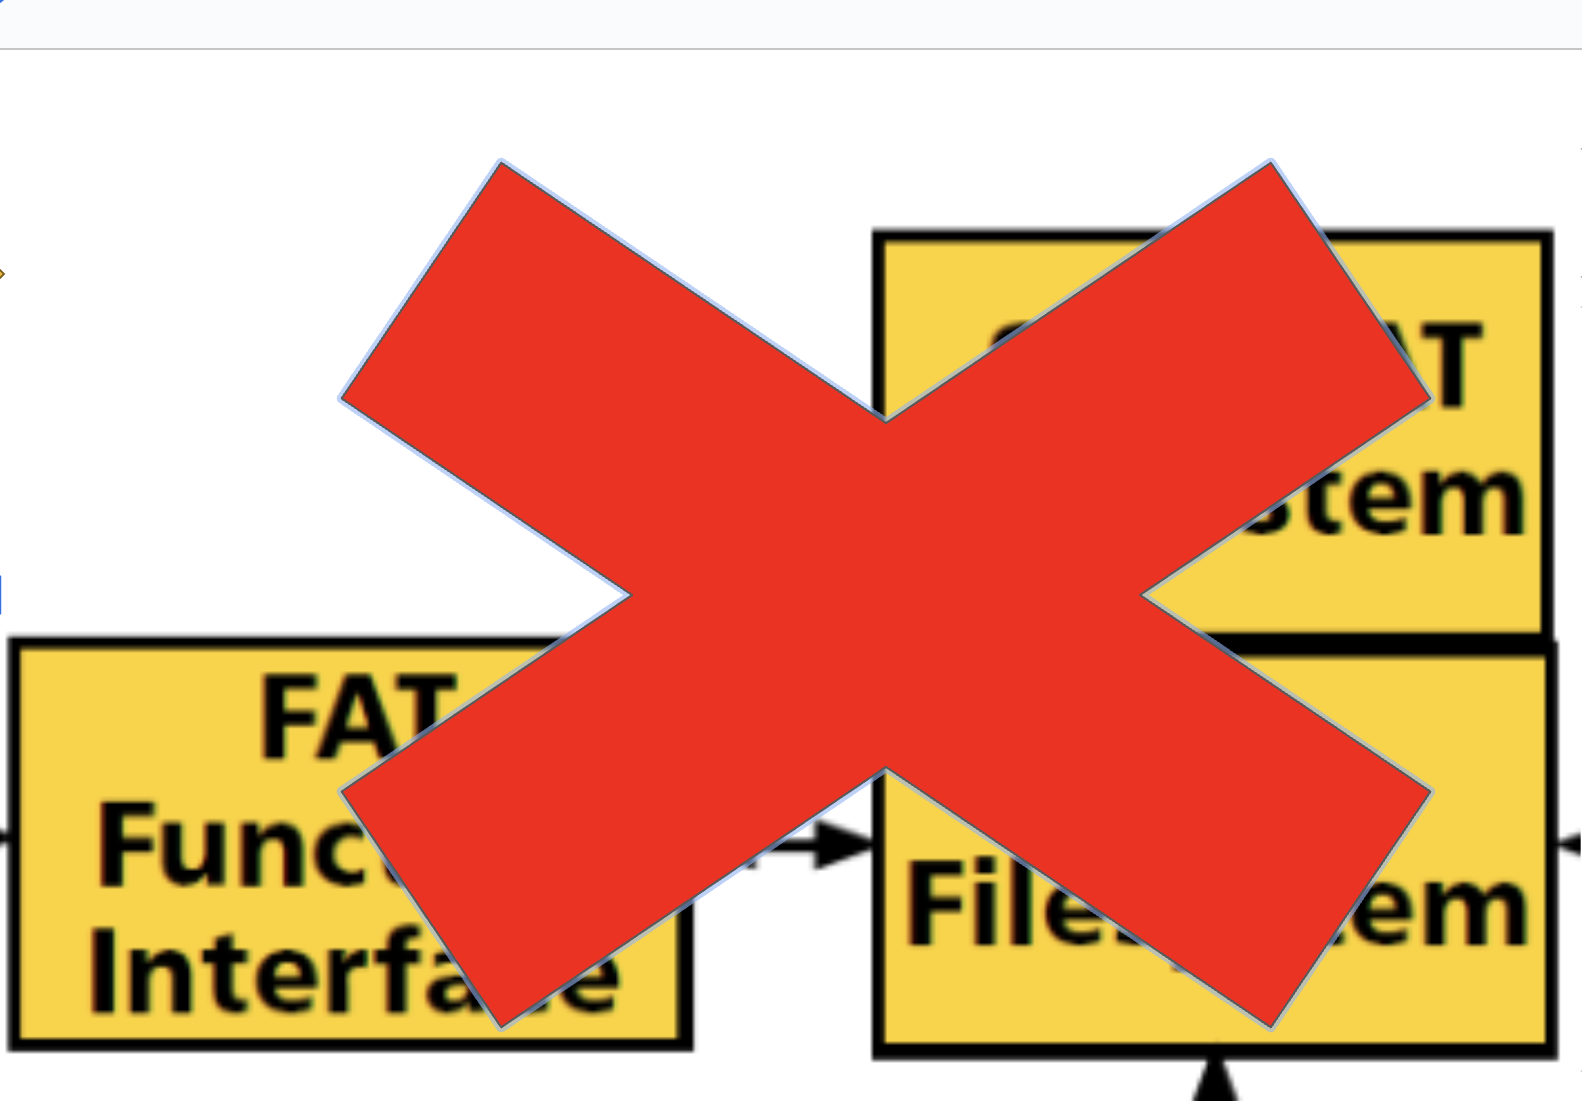
\includegraphics[height=0.4\textheight,width=0.5\textwidth,keepaspectratio]{images/safefat_x.png}
                \caption{SafeFAT integration}
            \end{figure}
        \end{column}
    \end{columns}  
\end{frame}

\begin{frame}{Lit Review: Possible Solutions}
    \begin{columns}
        \begin{column}{0.5\textwidth}
            \begin{itemize}
                \item \textbf{Error-Correcting Codes (ECC):} Detect and correct errors in data
                \item \textbf{File System Integration:} Integrating SafeFAT or ZFS to manage data integrity
                \item \textbf{Redundant Array of Independent Disks (RAID):} Use multiple disks to improve reliability
            \end{itemize}
        \end{column}
        \begin{column}{0.5\textwidth}
            \begin{figure}
                \centering
                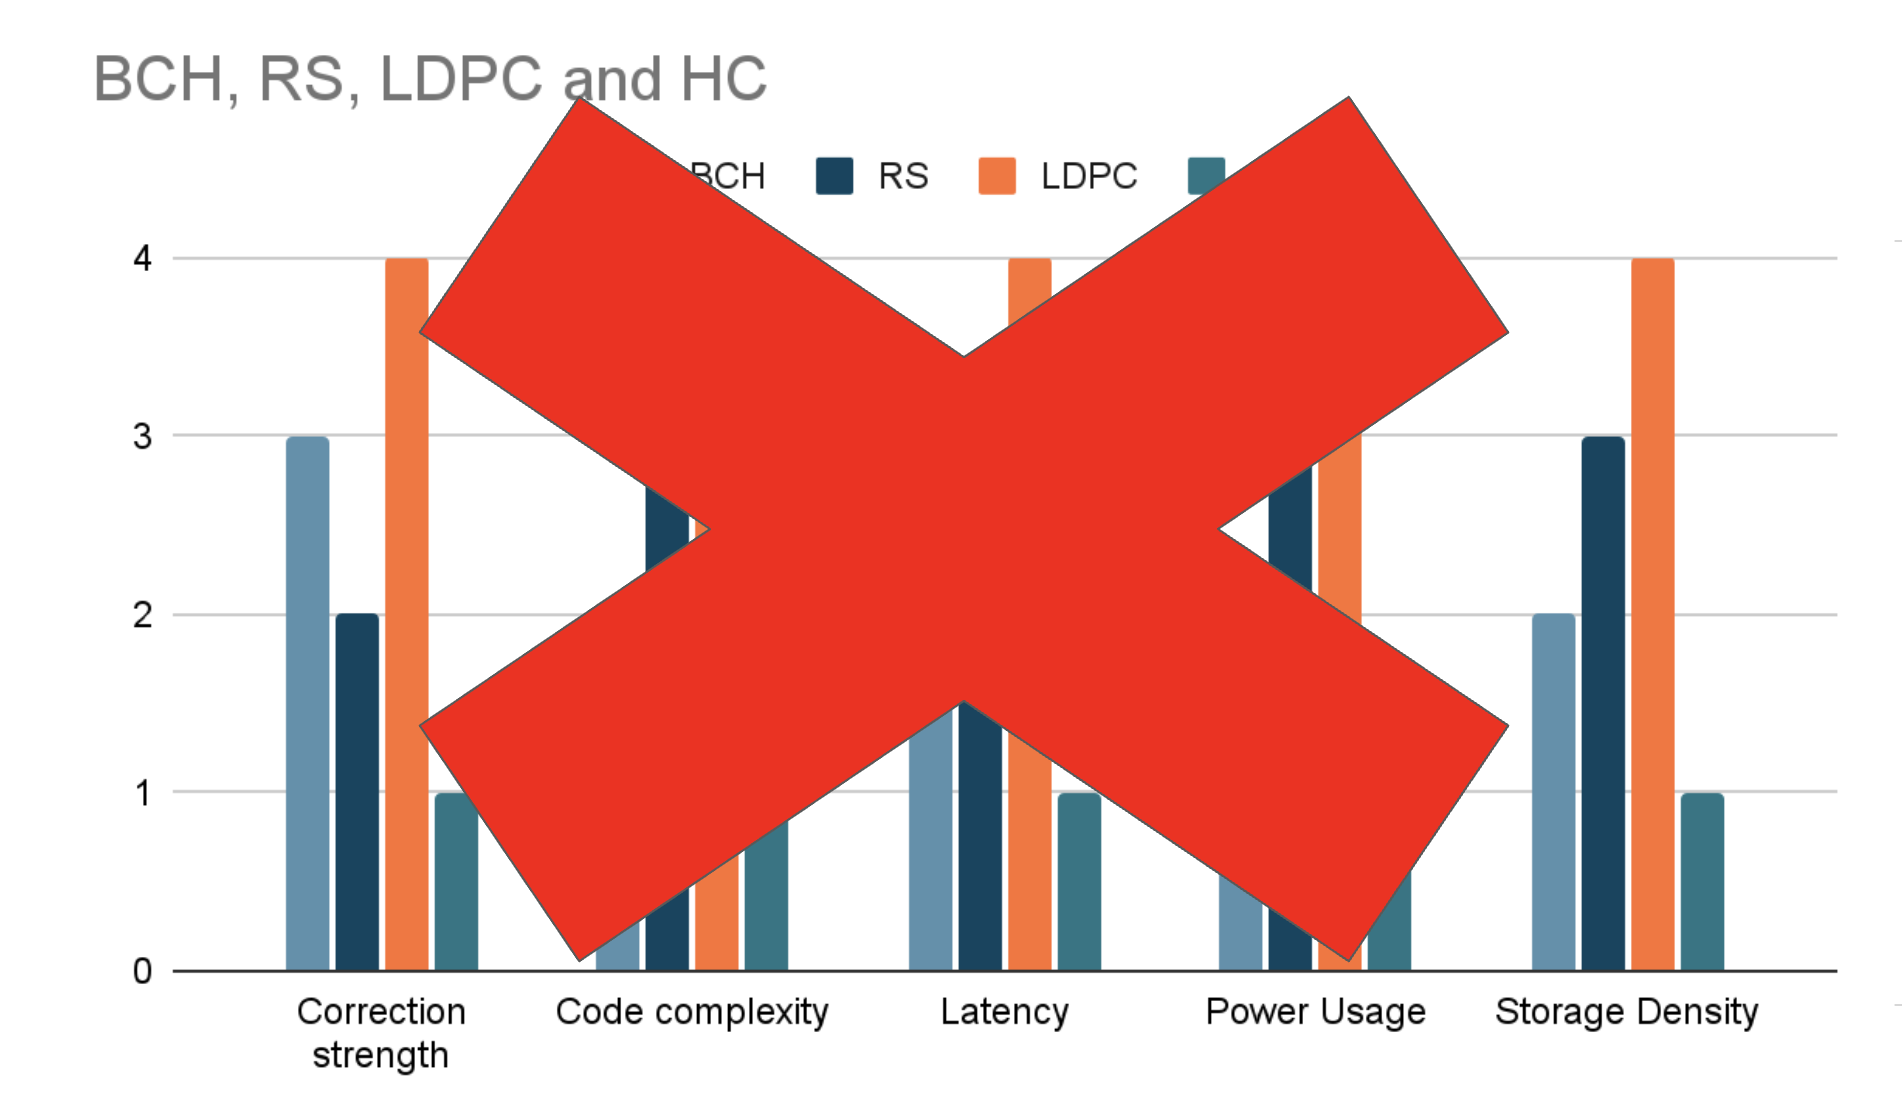
\includegraphics[height=0.4\textheight,width=0.5\textwidth,keepaspectratio]{images/ecc_x.png}
                \caption{Ranking of ECC (based on lit review)}
            \end{figure}
            \begin{figure}
                \centering
                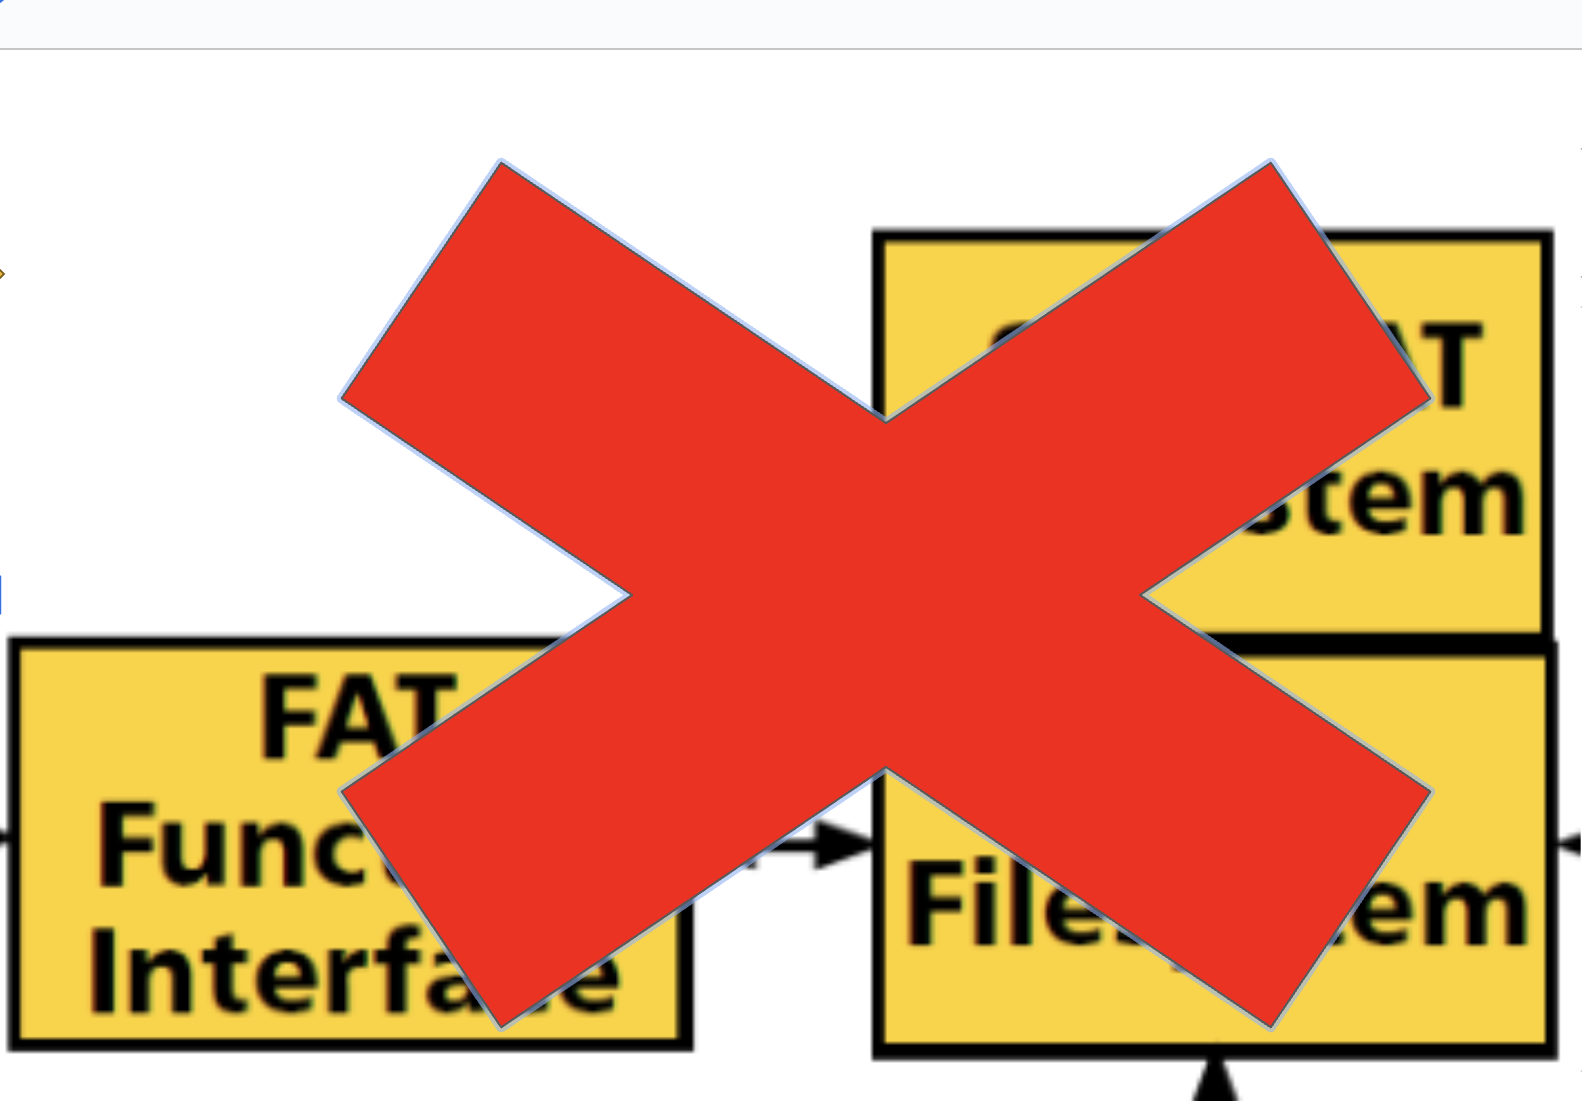
\includegraphics[height=0.4\textheight,width=0.5\textwidth,keepaspectratio]{images/safefat_x.png}
                \caption{SafeFAT integration}
            \end{figure}
        \end{column}
    \end{columns}  
\end{frame}

\begin{frame}{Lit Review: Possible Solutions}
    \begin{columns}
        \begin{column}{0.5\textwidth}
            \begin{itemize}
                \item \textbf{Error-Correcting Codes (ECC):} Detect and correct errors in data
                \item \textbf{File System Integration:} Integrating SafeFAT or ZFS to manage data integrity
                \item \textbf{Redundant Array of Independent Disks (RAID):} Use multiple disks to improve reliability
                \item \textbf{File Level Checksums:} Checksums at file level(CRC32, SHA-256)
            \end{itemize}
        \end{column}
        \begin{column}{0.5\textwidth}
            \begin{figure}
                \centering
                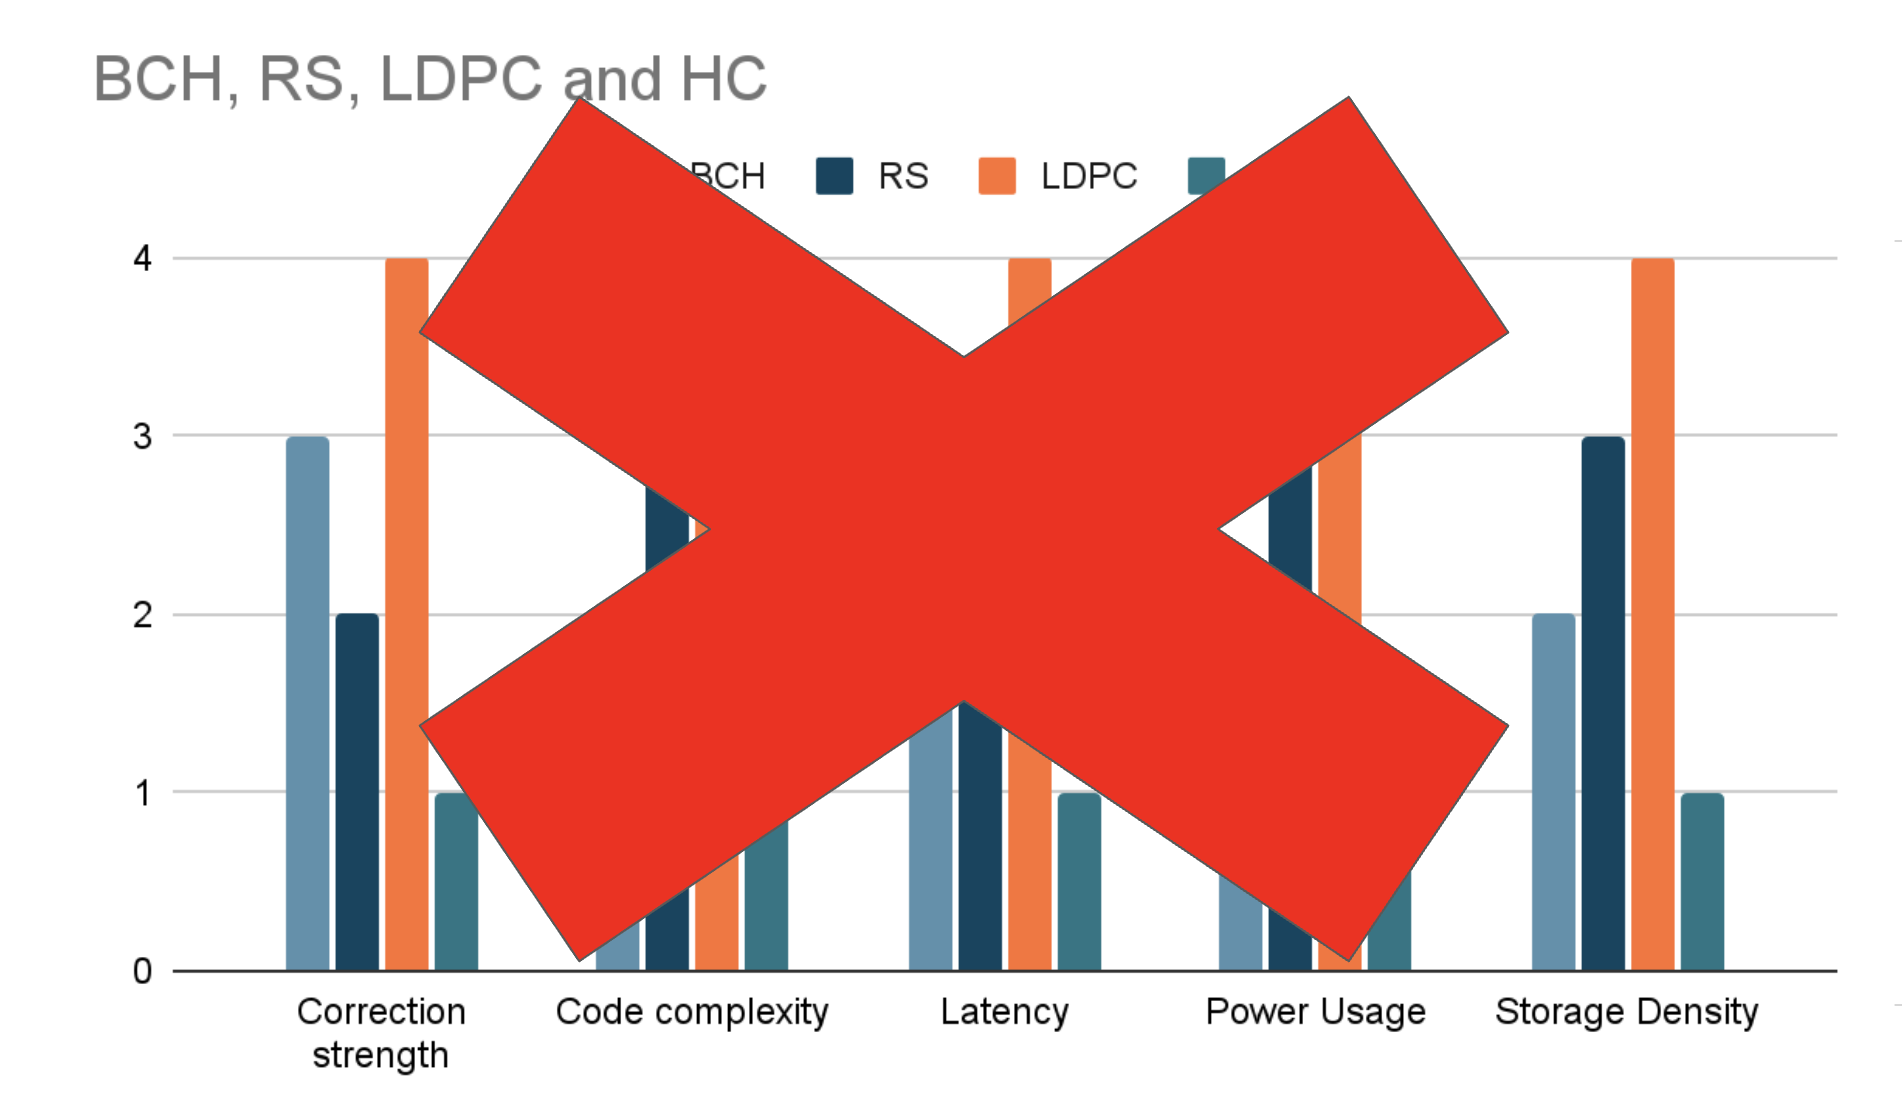
\includegraphics[height=0.4\textheight,width=0.5\textwidth,keepaspectratio]{images/ecc_x.png}
                \caption{Ranking of ECC (based on lit review)}
            \end{figure}
            \begin{figure}
                \centering
                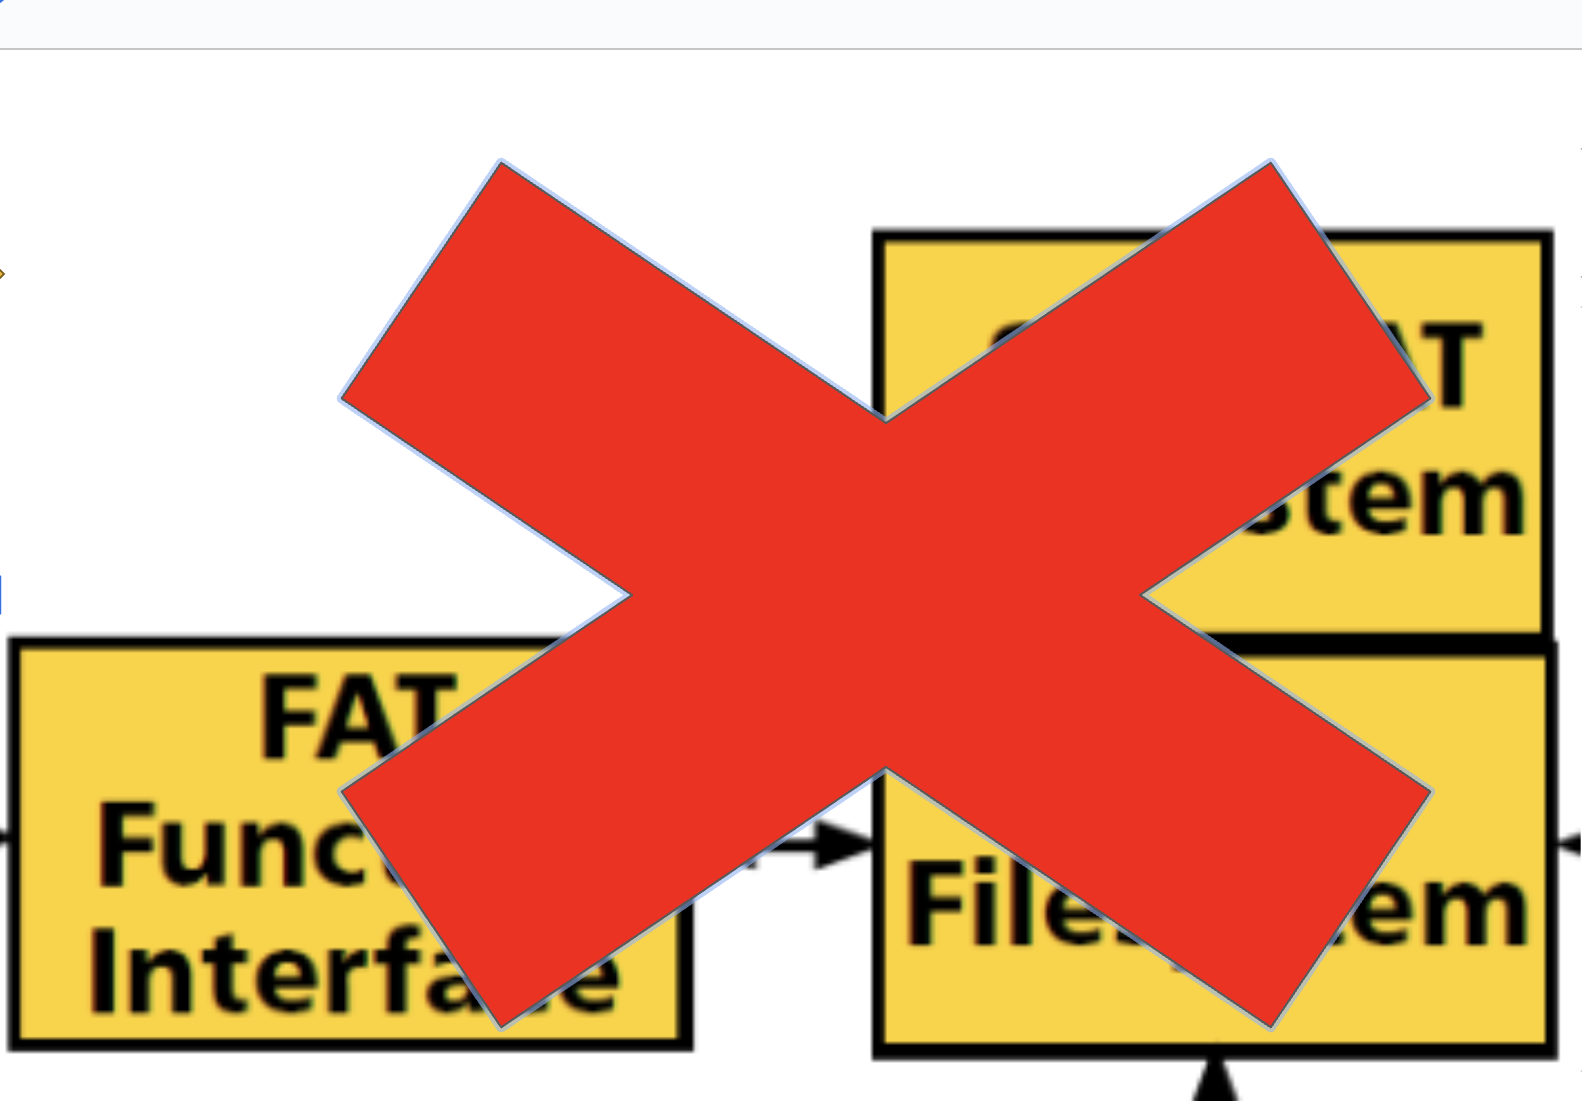
\includegraphics[height=0.4\textheight,width=0.5\textwidth,keepaspectratio]{images/safefat_x.png}
                \caption{SafeFAT integration}
            \end{figure}
        \end{column}
    \end{columns}  
\end{frame}

\begin{frame}{What's next?}
    \begin{itemize}
        \item Keep researching ways to minimize data loss (file level)
        \item Communicate with collaborators to clearly identify needs
        \item Visualize data loss rate
    \end{itemize}
\end{frame}
